\section{Comparação dos Algoritmos}
\label{sec:comparacao-algoritmos}

Nesta seção é apresentada a comparação experimental e teórica entre os quatro métodos
de busca implementados: Busca em Profundidade (DFS), Busca em Largura (BFS),
Busca de Custo Mínimo (UCS) e Busca A*. A análise contempla as métricas de qualidade da
solução (custo total da travessia em minutos), esforço computacional de exploração
(número de nós visitados/expandidos) e tempo de execução.

\subsection{Metodologia da comparação}
\label{subsec:metodologia}

Os experimentos foram conduzidos sobre a seguint instância  do problema da Ponte e da
Tocha, composta por quatro pessoas com os seguintes tempos individuais de travessia:

\begin{equation}
	P = \{A: 1\text{ min},\; B: 2\text{ min},\; C: 5\text{ min},\; D: 10\text{ min}\}.
\end{equation}

Como o espaço de estados desse problema é compacto e os tempos de busca individuais
ocorrem na escala de frações de milissegundo, medições isoladas sofrem influência
significativa de ruídos do sistema operacional (como escalonamento de processos e
efeitos de memória cache) e da ordem de iteração em estruturas de conjunto
(\texttt{set}) do Python. Para contornar essas flutuações, cada algoritmo foi executado
ao longo de \textbf{100 repetições independentes}.

As métricas registradas foram:
\begin{enumerate}
	\item \textbf{Custo do caminho}: soma dos tempos das ações que compõem a solução encontrada, expressa em minutos ($g(s_f)$).
	\item \textbf{Nós visitados}: contagem de nós efetivamente retirados da fronteira de busca para teste de objetivo e expansão de sucessores.
	\item \textbf{Tempo de processamento}: tempo decorrido de CPU durante a execução da busca, medido em milissegundos (ms) por meio da função \texttt{time.perf\_counter()}.
\end{enumerate}

Todos os ensaios foram realizados em ambiente Linux x86\_64 com interpretador Python 3.13.

\subsection{Resultados}
\label{subsec:resultados}

Os valores médios obtidos após as 100 execuções de cada algoritmo estão sumarizados na
Tabela~\ref{tab:comparacao-final}.

\begin{table*}[t]
	\centering
	\caption{Comparação das métricas médias obtidas ao longo de 100 repetições na instância $[1, 2, 5, 10]$.}
	\label{tab:comparacao-final}
	\begin{tabular}{lcccc}
		\toprule
		Algoritmo                   & Solução Ótima? & Custo Médio (min) & Nós Visitados & Tempo Médio (ms) \\
		\midrule
		Busca em Profundidade (DFS) & Não            & 50{,}21           & 10{,}64       & 0{,}195          \\
		Busca em Largura (BFS)      & Não            & 29{,}66           & 26{,}00       & 0{,}390          \\
		Busca de Custo Mínimo (UCS) & Sim            & 17{,}00           & 26{,}00       & 0{,}398          \\
		Busca A*                    & Sim            & 17{,}00           & 26{,}00       & 0{,}408          \\
		\bottomrule
	\end{tabular}
\end{table*}

\begin{figure}[H]
	\centering
	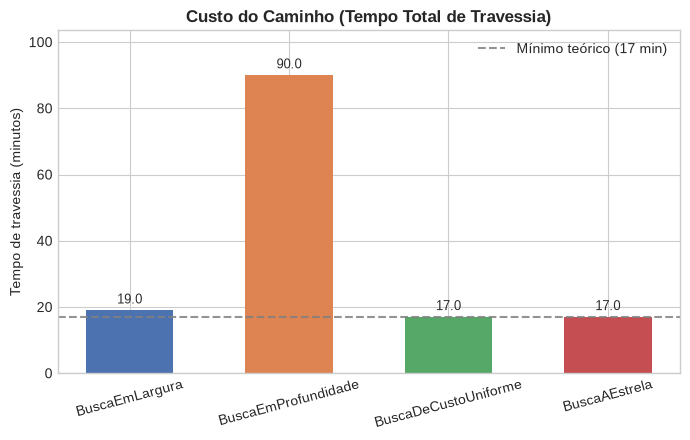
\includegraphics[width=\columnwidth]{results/grafico_custo.png}
	\caption{Comparação do tempo total de travessia (custo da solução) encontrado por cada algoritmo. A linha tracejada cinza indica o mínimo teórico ótimo de 17 minutos.}
	\label{fig:grafico-custo}
\end{figure}

\begin{figure}[H]
	\centering
	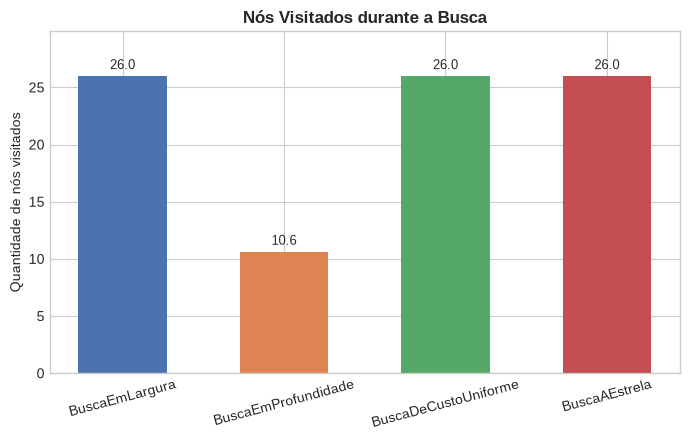
\includegraphics[width=\columnwidth]{results/grafico_nos_visitados.png}
	\caption{Quantidade média de nós visitados (expandidos da fronteira) até alcançar a solução.}
	\label{fig:grafico-nos}
\end{figure}

\begin{figure}[H]
	\centering
	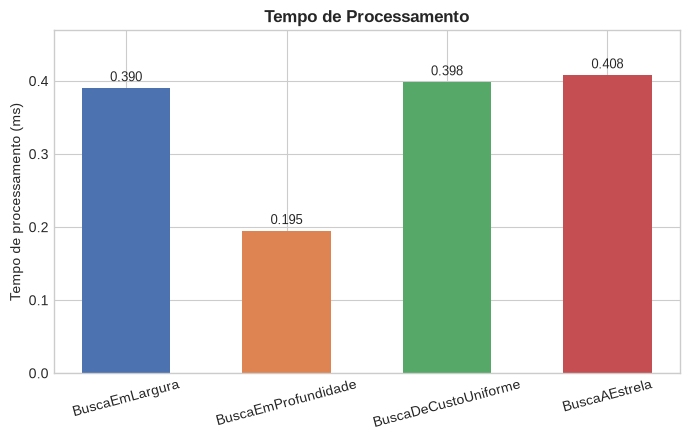
\includegraphics[width=\columnwidth]{results/grafico_tempo.png}
	\caption{Tempo médio de processamento por algoritmo expresso em milissegundos (ms).}
	\label{fig:grafico-tempo}
\end{figure}

\subsection{Discussão dos resultados}
\label{subsec:discussao}

A análise comparativa evidencia contrastes fundamentais na natureza e nas garantias
oferecidas por cada família de algoritmos:

\begin{itemize}[leftmargin=1.5cm]
	\item \textbf{Busca em Profundidade (DFS)}: Apresentou o menor tempo médio de CPU
	      ($0{,}195\text{ ms}$) e a menor média de nós visitados ($10{,}64$). No entanto, esse
	      desempenho computacional aparece por ter encontrado uma solução sub-ótima mais cedo,
	      como vemos que o custo médio da travessia foi de $50{,}21\text{ minutos}$, quase três
	      vezes superior ao tempo ótimo. Por priorizar a profundidade, a DFS mergulha no
	      primeiro ramo exploratório disponível e tende a retornar a pessoas que já haviam
	      atravessado, gerando travessias repetitivas e selecionando pares arbitrários e
	      lentos. Trata-se, portanto, de um método inadequado quando o critério de sucesso
	      envolve a minimização do tempo de travessia.

	\item \textbf{Busca em Largura (BFS)}: Explorou exatamente $26{,}00\text{ nós}$ na
	      média, com tempo de execução de $0{,}390\text{ ms}$. A BFS cumpre estritamente sua
	      propriedade teórica de encontrar a solução com o \textbf{menor número de passos}
	      (5 travessias no total). Entretanto, o custo médio obtido foi de
	      $29{,}66\text{ minutos}$, consideravelmente acima do ótimo. Como a BFS é cega em
	      relação ao tempo dos participantes, ela frequentemente escolhe uma sequência de
	      5 passos que não emparelha os indivíduos mais lentos de forma estratégica.

	\item \textbf{Busca de Custo Mínimo (UCS)}: Encontrou o custo ótimo de
	      $17{,}00\text{ minutos}$ em 100\% dos ensaios, consumindo $0{,}398\text{ ms}$ e
	      visitando $26{,}00\text{ nós}$. Ao guiar sua fronteira pela função $g(n)$,
	      o algoritmo assegura que nenhum estado com custo acumulado superior a 17 seja
	      considerado antes do estado objetivo ideal.

	\item \textbf{Busca A*}: Também alcançou a solução ótima de
	      $17{,}00\text{ minutos}$, visitando $26{,}00\text{ nós}$ em $0{,}408\text{ ms}$.
	      A igualdade na quantidade de nós visitados entre A* e UCS decorre da dimensão
	      compacta do espaço de estados do problema: com 4 pessoas, o grafo possui no
	      total apenas 32 estados possíveis (dos quais 26 são alcançáveis até a profundidade
	      da solução). Como a estratégia ótima exige enviar as pessoas mais lentas juntas
	      ($C$ e $D$, gastando 10 min) e trazer de volta uma pessoa rápida ($A$ ou $B$), a
	      heurística $h_{\max}$, baseada exclusivamente na pessoa mais lenta remanescente na
	      origem, atinge seu valor máximo logo no início e não introduz podas adicionais no
	      reduzido volume de estados intermediários. Em instâncias com maior número de pessoas,
	      o A* passaria a podar significativamente mais estados do que a UCS graças ao
	      direcionamento fornecido por $h(n)$.
\end{itemize}

\subsection{Por que a Busca em Largura não garante a solução de menor tempo?}
\label{subsec:por-que-bfs-nao-garante-otimo}

A razão pela qual a Busca em Largura (BFS) não garante a solução ótima em tempo total
decorre da diferença fundamental entre \textbf{otimação do número de arestas} e
\textbf{otimação do custo do caminho (soma ponderada das arestas)}.

A BFS pressupõe que todas as arestas do grafo possuem custo idêntico ou unitário
($c(u, v) = 1$). Sob essa premissa, o caminho com menor número de passos será
necessariamente o caminho de menor custo. Contudo, no Problema da Ponte e da Tocha, o
grafo é ponderado com custos não uniformes determinados por $c(M) = \max_{p \in M} t(p)$,
o que faz com que encontre uma solução sub-ótima primeiro e por isso não explore outras
soluções alternativas.

No problema com $P = [1, 2, 5, 10]$, o número mínimo absoluto de travessias para levar 4 pessoas de um lado ao outro em uma ponte de capacidade 2 é de \textbf{5 passos} (três idas e duas voltas). Existem múltiplos caminhos distintos no grafo que alcançam o objetivo em exatamente 5 passos, por exemplo:

\begin{enumerate}
	\item \textbf{Caminho Subótimo em 5 passos}:
	      \begin{itemize}
		      \item Passo 1: $A$ e $D$ vão $\implies$ custo $\max(1, 10) = 10\text{ min}$.
		      \item Passo 2: $A$ volta $\implies$ custo $1\text{ min}$.
		      \item Passo 3: $A$ e $C$ vão $\implies$ custo $\max(1, 5) = 5\text{ min}$.
		      \item Passo 4: $A$ volta $\implies$ custo $1\text{ min}$.
		      \item Passo 5: $A$ e $B$ vão $\implies$ custo $\max(1, 2) = 2\text{ min}$.
	      \end{itemize}
	      Custo acumulado total: $10 + 1 + 5 + 1 + 2 = \mathbf{19\text{ minutos}}$ (ou valores ainda maiores, como 29 ou 37 min, se pessoas mais lentas retornarem com a tocha).

	\item \textbf{Caminho Ótimo em 5 passos}:
	      \begin{itemize}
		      \item Passo 1: $A$ e $B$ vão $\implies$ custo $\max(1, 2) = 2\text{ min}$.
		      \item Passo 2: $A$ volta $\implies$ custo $1\text{ min}$.
		      \item Passo 3: $C$ e $D$ vão juntos $\implies$ custo $\max(5, 10) = 10\text{ min}$.
		      \item Passo 4: $B$ volta $\implies$ custo $2\text{ min}$.
		      \item Passo 5: $A$ e $B$ vão $\implies$ custo $\max(1, 2) = 2\text{ min}$.
	      \end{itemize}
	      Custo acumulado total: $2 + 1 + 10 + 2 + 2 = \mathbf{17\text{ minutos}}$.
\end{enumerate}

Como ambos os caminhos possuem exatamente profundidade 5, ambos pertencem ao mesmo nível na árvore de busca da BFS. Como a BFS organiza sua fronteira exclusivamente pela ordem de chegada dos nós na fila FIFO, o primeiro estado objetivo desenfileirado dependerá unicamente da ordem arbitrária em que os sucessores foram gerados e inseridos na fila -- e não do tempo acumulado. Por isso, a BFS frequentemente retorna uma solução de 19, 29 ou mais minutos.

Em contrapartida, a \textbf{Busca de Custo Mínimo} organiza a fronteira em ordem crescente de $g(n)$, e a \textbf{Busca A*} organiza por $f(n) = g(n) + h(n)$. Sendo todos os custos de aresta não negativos e sendo a heurística $h(n)$ admissível (ou seja, $h(n) \leq h^*(n)$), ambos os algoritmos possuem a garantia matemática formal de que nenhum nó com custo real superior a 17 minutos será expandido antes que o caminho de custo mínimo seja selecionado, garantindo a solução ótima.
